\section{Grammar Definition}
This is the grammar definition used to generate descriptions from the probability distribution over words estimated by the model.
Note however, that no grammar was used in learning: the speech recognizer used as frontend to the spoken descriptions is based on a loop of words with no grammar, and the affordance-word model is based on a bag-of-word assumption where only the presence of absence of each word in the description is considered.

\begin{figure}
  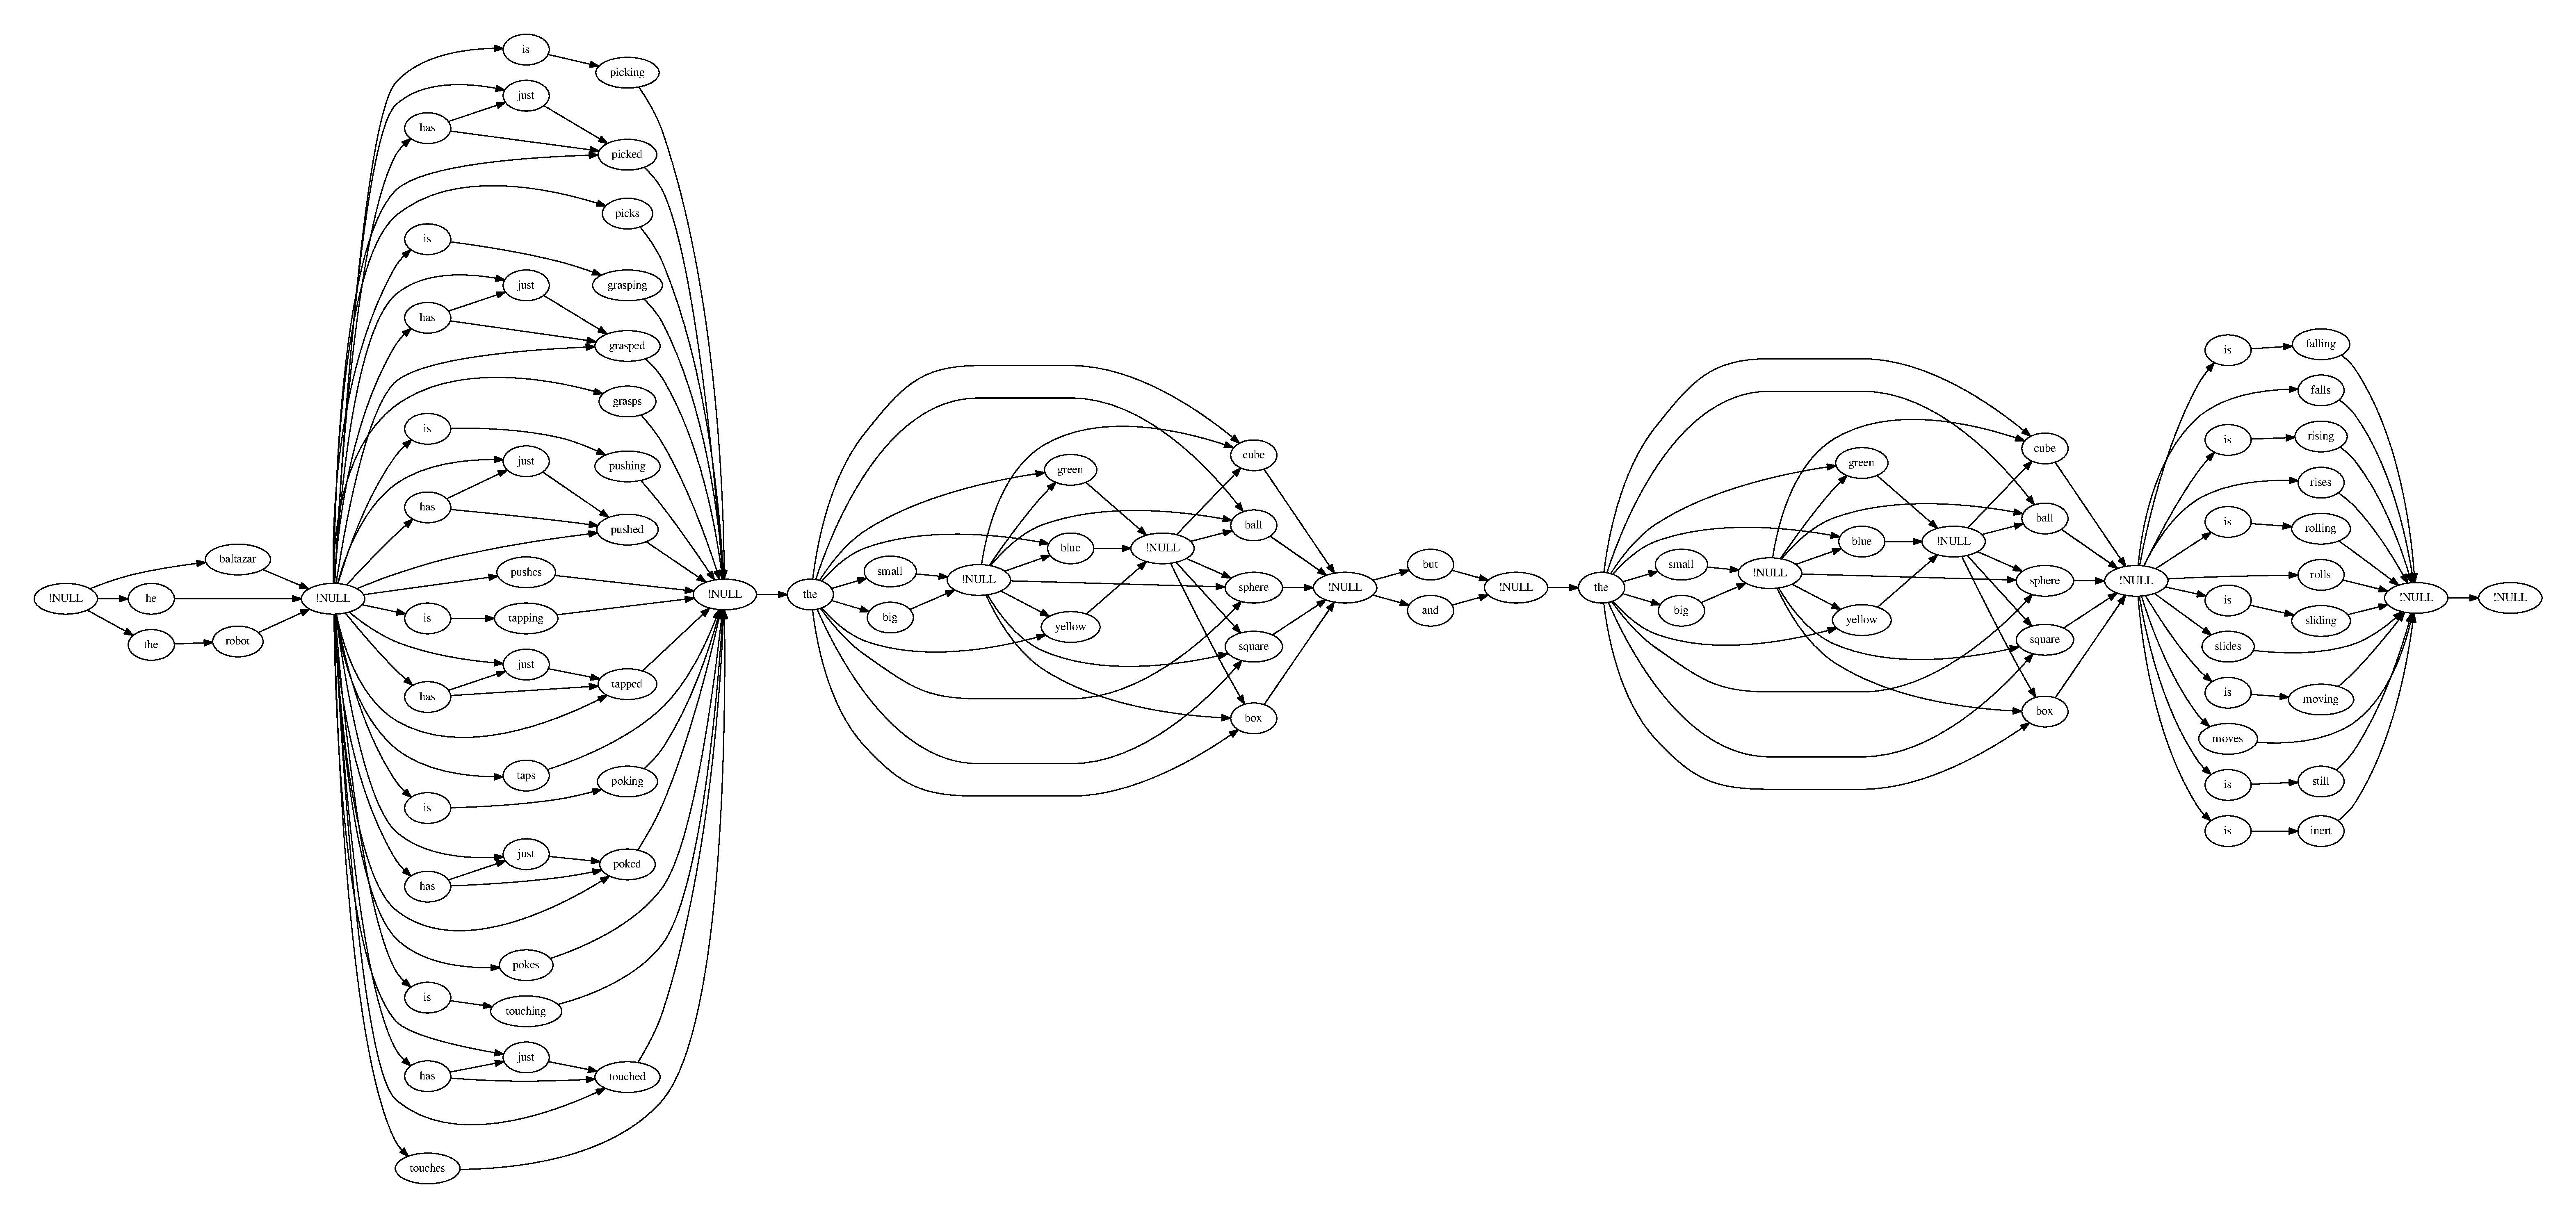
\includegraphics[width=\textwidth, angle=90]{figures/grammar}
  \caption{Graphical representation of the formal context-free grammar used to generate descriptions from word probability distribution.}
\end{figure}

\begin{grammar}
  <agent> ::= the robot | he | baltazar 

  <size> ::= big | small
  
  <color> ::= green | yellow | blue
  
  <shape> ::= sphere | ball | cube | box | square
  
  <object> ::= the [<size>] [<color>] <shape>
  
  <touch> ::= touches | [has] [just] touched | is touching
  
  <poke> ::= pokes | [has] [just] poked | is poking
  
  <tap> ::= taps | [has] [just] tapped | is tapping
  
  <push> ::= pushes | [has] [just] pushed | is pushing
  
  <grasp> ::= grasps | [has] [just] grasped | is grasping
  
  <pick> ::= picks | [has] [just] picked | is picking
  
  <action> ::= <touch> | <poke> | <tap> | <push> | <grasp> | <pick>
  
  <conjunction> ::= and | but
  
  <inertmove> ::= is inert | is still | moves | is moving
  
  <slideroll> ::= slides | is sliding | rolls | is rolling
  
  <fallrise> ::= rises | is rising | falls | is falling
  
  <effect> ::= <inertmove> | <slideroll> | <fallrise>
  
  <sentence> ::= <agent> <action> <object> <conjunction> <object> <effect>
\end{grammar}

Given a probability distribution over the words $P(w_i)$, a number $N$ of sentences is randomly generated from the grammar using the \texttt{HSGen} tool from HTK.
Then the sentences are rescored according to the log likelihood of each words in the sentence normalized by the lenght of the sentence.
Finally an n-best list of possible descriptions is produced by sorting the scores.

\begin{equation*}
  \text{score}(s_j) = \frac{1}{n_j} \sum_{k=1}^{n_j} \log P(w_{jk}),
\end{equation*}
where $s_j$ is the $j$th sentence, $n_j$ is the number of words in sentence $s_j$ and $w_{jk}$ is the $k$th word in sentence $s_j$.

